%\addbibresource{/home/jorgsk/Dropbox/phdproject/bibtex/jorgsk.bib}
\subsection{Model of initial transcription}
Our model describes the process of initial transcription by considering the
following reactions i) NAC ii) backtracking iii) unscrunching and abortive
RNA release (UAR), and iv) promoter escape (Figure
S\ref{fig:model_and_rates}A). Here, we consider backtracking as the first
unscrunching step, also known as backstepping; this rate constant is unique in
that it is obtained using experimentally obtained abortive probabilities
(APs) \cite{hsu_quantitative_1996}. To obtain the rate constant of
backtracking, we make use of the model constraint that the NAC and
backtracking are in kinetic competition, and assume that the probability to
backtrack at any given template position is equal to the AP at that
position, implying that all backtracking events lead to an aborted RNA. In
combination,
\begin{equation*}
    \frac{b_i}{b_i + \text{NAC}_i} = \text{AP}_i,
\end{equation*}
where subscript $i$ indicates position, and NAC and $b$ are the rate constants
the nucleotide addition cycle and backtracking, respectively. From this
expression, we obtain the rate constant for backtracking given a rate constant
of the NAC and an AP:
\begin{equation}
  b_i = \frac{\text{NAC}_i\cdot\text{AP}_i}{1-\text{AP}_i}.
  \label{eq:backtrackingcalc}
\end{equation}
Figure~S\ref{fig:model_and_rates}B shows the initial transcription kinetic
reaction diagram with the rate constants to be estimated, and
Figure~S\ref{fig:backtracking_calc_example} shows example calculations of rate
constants from backtracking.

In this work we apply the model using APs obtained both for the absence of
GreB (-GreB) and in the presence of GreB (+GreB). When GreB is present,
backtracked complexes may be rescued by GreB stimulated cleavage of the
unaligned 3\ppp end of the transcript. Therefore, APs obtained in the presence
of GreB represent the probability to both backtrack and to avoid rescue by
GreB until abortive RNA release. We assume that GreB-mediated cleavage and
subsequent NACs are rapid steps compared to unscrunching, using the APs
obtained in the presence of GreB as effective backtracking probabilities. All
AP values are obtained from Hsu et al. \cite{hsu_initial_2006}.

\subsection{Implementation and parameter estimation}
The rate constants in the model is obtained by fitting to experimental data.
The data used for rate constant estimation is the distribution of time spent
in abortive cycling \cite{revyakin_abortive_2006}. This data was obtained from
100 individual initial transcription events. For experiments with single
molecules, there is an inherent stochastic component in the experimental
outcome that derives from the randomness of molecular motion. This can be seen
as the speed of transcription elongation obtained by single-molecule
experiments show large standard deviations \cite{adelman_single_2002,
tolic-norrelykke_diversity_2004}. To account for this randomness, we perform
the kinetic simulations using the direct method of the Gillespie algorithm for
stochastic simulations of chemical reactions \cite{gillespie_exact_1977}.
Specifically, we make use the version implemented by Maarleveld et al.\ in the
StocPY software \cite{maarleveld_stochpy:_2013}.

We estimate the rate constants using the following procedure (rate constants
given in Figure S1): First, we assign random values to the three rate
constants NAC ($k_n$), promoter escape ($k_e$) and unscrunching and abortive
RNA release ($k_u$) within certain fixed boundaries (see below). These values
are chosen independently from a uniform distribution. Secondly, we calculate
the rate constant of backtracking ($k_b$) using equations
\ref{eq:backtrackingcalc}. We then simulate 100 initial transcription events
and calculate the distribution of time spent in abortive cycling as a result
of these specific rate constants. The resulting time spans are compared to
empirical values \cite{revyakin_abortive_2006} using the root mean square
error (RMSE). By repeating this procedure many times, we obtain statistics of
which combinations of rate constants lead to model results with minimal
deviation compared to the experimental outcome.

The boundaries of the rate constants were chosen based on experimental
evidence. We assumed that the rate constant of the NAC would not surpass 25
s$^{-1}$ \cite{??}. From single molecule experiments, it is known that the
rate constants of the assumed slowest step, unscrunching and abortive RNA
release, must be faster than 1 s$^{-1}$, since this was the time-resolution of
the experimental equipment \cite{revyakin_abortive_2006}; similarly, promoter
escape should be faster than 1 s$^{-1}$. We therefore set the minimum and
maximum values of all rate constants to be 1 s$^{-1}$ and 25 s$^{-1}$,
respectively. 

\begin{figure}
	\begin{center}
        \includegraphics{/home/jorgsk/Dropbox/The-Tome/my_papers/kinetic_initiation/illustrations/model_and_rates.pdf}
	\end{center}
    \caption{Kinetic model scheme and reaction rate constants. \textbf{A})
    From the open complex (OC) transcription proceeds by nucleotide additions
    cycles from one initial transcribing complex (IC) to the next, where each
    IC is identified in subscript by the length of its nascent RNA. Initial
    transcription proceeds until the nascent RNA has reached the
    experimentally obtained maximum size of abortive transcript (MSAT)
    \cite{hsu_initial_2006}. For ICs with an RNA of 2 nt in length or longer, there is a
    competition between the nucleotide addition cycle (NAC) and backtracking.
    Backtracking causes termination of transcription, and only further
    backtracking (unscrunching) and abortive RNA release may follow, returning
    RNAP to the open complex. From the open complex forward transcription may
    resume once more. \textbf{B}) Kinetic reactions diagram containing the
    rate constants NAC (denoted here as $k_n$), promoter escape (denoted as
    $k_e$) and unscrunching and abortive release ($k_u$), as well as the rate
    constants of backtracking, $k_{b,i}$.}
    \label{fig:model_and_rates}
\end{figure}
